%! Author = annam
%! Date = 10/01/2023

% Preamble
\documentclass[11pt]{article}

% Packages
\usepackage{amsmath}

% Document
\begin{document}
\section{Ziel}
In diesem Versuch liegt die Zielsetzung in der Vermessung von Magnetfeldstärken bei verschiedenen Anordnungen von Spulen.
Dafür werden zwei einzelne Spulen, ein Spulenpaar und eine Ringspule verwendet.

\section{Theoretische Grundlagen}
Dem Versuch zugrundeliegend ist die Entstehung von Magnetfeldern durch bewegte Ladungen.
Das entstehende Feld kann durch seine Eigenschaften beschrieben werden, die sich allgemein als vektorielle Größen
darstellen lassen.

\subsection{Feldstärke, Flussdichte \& Biot-Savart Gesetz}
Eine Größe ist die magnetische Feldstärke $\vec{H}$, anhand welcher sich der Betrag und die Ausrichtung des Feldes
bestimmen lassen.
\begin{figure}
    \centering
    \includegraphics[width=0.3\textwidth]{Bildschirmfoto 2022-12-02 um 21.17.02.png}
    \caption{Graphische Darstellung eines Magnetfeldes um einen Stromdurchflossenen Leiter \cite{anleitung}.}
\end{figure}
Um das Magnetfeld anschaulich zu visualisieren werden Magnetfeldlinien verwendet, vergleichbar mit einem elektrischen Feld.
Die Linien verlaufen in tangentialer Richtung zu $\vec{H}$ und sind, im Gegensatz zum elektrischen Pendant, geschlossen.
Für einige Atome, ohne Einfluss eines äußeren Magnetfeldes, besteht ein Zusammenhang zwischen der Feldstärke, der
Permeabilität \mu und der magnetischen Flussdichte $\vec{B}$.
Unter der Flussdichte wird hierbei die Stärke des magnetischen Flusses durch ein beliebiges Flächenelement verstanden und
verläuft somit in Richtung der Feldlinien.
Der Zusammenhang ist gegeben als
\begin{equation}
    \vec{B} = \mu\cdot\vec{H},\notag
    \end{equation}
wobei mit der Permeabilität das Produkt der Vakuum-Permeabilität $\mu_{0}$ und der materialspezifischen Permeabilität
$\mu_{r}$ gemeint ist.
Bei Betrachtung eines stromdurchflossenen Leiters anstelle einer Einzelladung überträgt sich der Zusammenhang auf ein
Magnetfeld, welches den Leiter in konzentrischen Kreisen umgibt.
So lässt sich nun bezogen auf einen beliebigen Leiterdraht die Feldstärke im Abstand $r$ zum Leiter über das Differential
der magnetischen Flussdichte beschreiben als
\begin{equation}
    d\vec{B} = \frac{\mu_{0}I}{4\pi} \frac{d\vec{s}}{\vec{r}\times{r^3}}\notag
    \end{equation}
mit dem Strom $I$ durch den Draht.
Diese Gleichung nennt sich Biot-Savart Gesetz.
Es kann zur Berechnung des Magnetfeldes bei komplexeren Verhältnissen, etwa einer Spule, verwendet werden.
Die Flussdichte in der Mitte einer Ringspule lässt sich damit beschreiben als
\begin{equation}
    \vec{B} = n \cdot \frac{\mu_{0}I}{2}\frac{R^2}{(R^2 + x^2)^{\frac{3}{2}}}\cdot\^{x} . \label{eq:BFeld} ,
    \end{equation}
wobei $n$ die Windungszahl der Spule meint.
\subsection{Homogene Felder}
Ist eine Spule sehr langgestreckt, dann kann die Feldstärke im mittleren Bereich als konstant angesehen werden und die
Feldlinien sind parallel.
Das Feld wird innerhalb dieses Bereichs homogen genannt und es gilt ein Proportionalitätszusammenhang zur Spulenlänge $l$,
der Windungszahl $n$ und dem Strom $I$ und wird berechnet durch
\begin{equation}
    B = \mu_{0}\mu_{r}\frac{n}{l}I .\notag
     \end{equation}
Wird die Spule zu einem Ring, eine Toroid, gebogen, dann ist das Feld innerhalb der Spule weiterhin homogen und außerhalb
null, während die Länge ersetzt wird durch $l = 2\pi r_{T}$.
\subsection{Helmholtz-Spulenpaar}
Als Helmholtz-Spule wird eine Anordnung von zwei Ringspulen mit gleicher Windungszahl bezeichnet, die auf der selben
Achse parallel aufgestellt sind und in gleichsinniger Richtung von einem Strom $I$ durchflossen werden.
Relevant dabei ist der Abstand zwischen den Spulen, der in diesem Falle dem Radius gleicht.
Dieser Aufbau ermöglicht die Entstehung eines weitesgehend homogenen Feldes zwischen den Spulen nahe der Symmetrieachse.
\begin{equation}
    B(0) = B_{1}(x) + B_{1}(ac{\mu_{0}IR^2}{(R^2+x^2)^{\frac{3}{2}}}.
    \end{equation}
Aus dem Biot-Savart Gesetz lässt sich das Feld in der Mitte (im Ursprung $x=0$) mit einer Spulenwindung herleiten und
der Feldgradient an der Symmetrieachse ergibt sich zu
\begin{equation}
    \frac{dB}{dx} = -3\mu_{0}IR^2 \cdot \frac{x}{(R^2+x^2)^{\frac{5}{2}}} .
    \end{equation}
\subsection{Ferromagnetismus}
Als Ferromagneten sind Materialien definiert, die auch ohne ein äußeres Magnetfeld ein permanentes magnetisches Moment
erzeugen.
Magnetische Momente können auf verschiedene Arten zueinander ausgerichtet beziehuungsweise polarisiert sein.
Den Sonderfall bei paralleler Ausrichtung (gleicher Polarisation) wird der Bereich als Weiß'scher Bezirk bezeichnet.
Diese treten typischerweise bei ferromagnetischen Materialien auf.
Sind die Ferromagneten unmagnetisiert, sind die Weiß'schen Bezirke klein und dessen Ausrichtung statistisch verteilt.
Wird nun ein äußeres Feld angelegt, gleichen sich die Richtungen mit der Zeit an und die Weiß'schen Bezirke vergrößern sich,
bis alle magnetischen Momente dieselbe Ausrichtung haben wie das Magnetfeld außen.
Da sie relative Permeabilität $\mu_{r}$ eines Ferromagneten sehr hoch ist herrscht für die Flussdichte keine Linearität mehr.
Verdeutlicht wird dieser Zusammenhang durch die Hysterese.
Hysterese bezeichnet den Effekt der Sättigung der Magnetisierung eines Ferromagneten bei Erhöhung oder Reduktion des
äußeren Magnetfeldes.
So verbleibt beispielsweise sogar noch Magnetisierung, wenn gar kein äußeres Feld mehr angelegt ist, was als Remanenz
bezeichnet wird.
Die Permeabilität wird also umdefiniert in Abhängigkeit der magnetischen Feldstärke $H$ und wird differentielle
Permeabilität $\mu_{diff}$ genannt.
Sie berechnet sich durch
\begin{equation}
    \mu_{\text{diff}} = \frac{1}{\mu_{0}\frac{dB}{dH}} .
    \end{equation}
\begin{figure}
    \centering
    \includegraphics[width=0.4\textwidth]{Pics/Bildschirmfoto 2022-12-02 um 21.16.49.png}
    \caption{Hysteresekurvenverlauf mit wichtigen Kenngrößen\cite{anleitung}.}
\end{figure}
\noindent
\noindent Wird nun ein ferromagnetischer Stoff in eine Spule gelegt, so erhöht sich durch seine Eigenschaften der
magnetische Fluss und die Feldstärke, wobei diese proportional von der Magnetisierung $\vec{M}$ abhängt.
Der magnetische Fluss ergibt sich dann zu
\begin{equation}
    \vec{B} = \mu_{0}(\vec{H} + \vec{M}) ,
    \end{equation}
mit $\vec{H}$ aus dem $\vec{H_{0}}$ im homogenen Bereich und $\vec{H_{R}}$ der Randeffekte zusammengesetzt.
Die Randeffekte können vermieden werden bei Bildung eines Toroids, sodass das $\vec{H_{R}}$ entfällt.
Aufgrund der hohen relativen Permeabilität ist die Magnetisierung wesentlich höher als die Feldstärke und diese kann in
der Gleichung vernachlässigt werden.
Es gilt für den magnetischen Fluss dann $\vec{B} \approx \mu_{0} \cdot \vec{M}$ .

\section{Versuchsaufbau}
Es werden für die Aufbauten verschiedene Spulentypen, Hallsonden und Netzgeräte benötigt.
Relevant vor Beginn der Messungen ist, dass noch keine Spannung angelegt wird und kein Strom fließt.
Die Funktionsweise der Sonden basiert auf dem Hall-Effekt.
Dieser beschreibt die entstehende Hall-Spannung bei stromdurchflossenen Leitern in einem homogenen Magnetfeld, dessen
Ausrichtung orthogonal sowohl zur Stromrichtung, als auch zur Magnetfeldausrichtung steht.
Dazu befindet sich an der Spitze der Sonde ein Leiterplättchen, an dem ein Strom angelegt wird, der senkrecht zu einem
Magnetfeld steht, sodass die Lorentzkraft auf die Ladungen wirkt.
Durch diese Kraft entsteht ein Verschiebungsstrom, welcher die Spannung veranlasst.
In dem Versuch werden zwei verschiedene Arten der Sonden verwendet, um die magnetische Feldstärke zu messen.
Diese sind eine transversale und eine longitudinale Hall-Sonde.
\begin{figure}
    \centering
    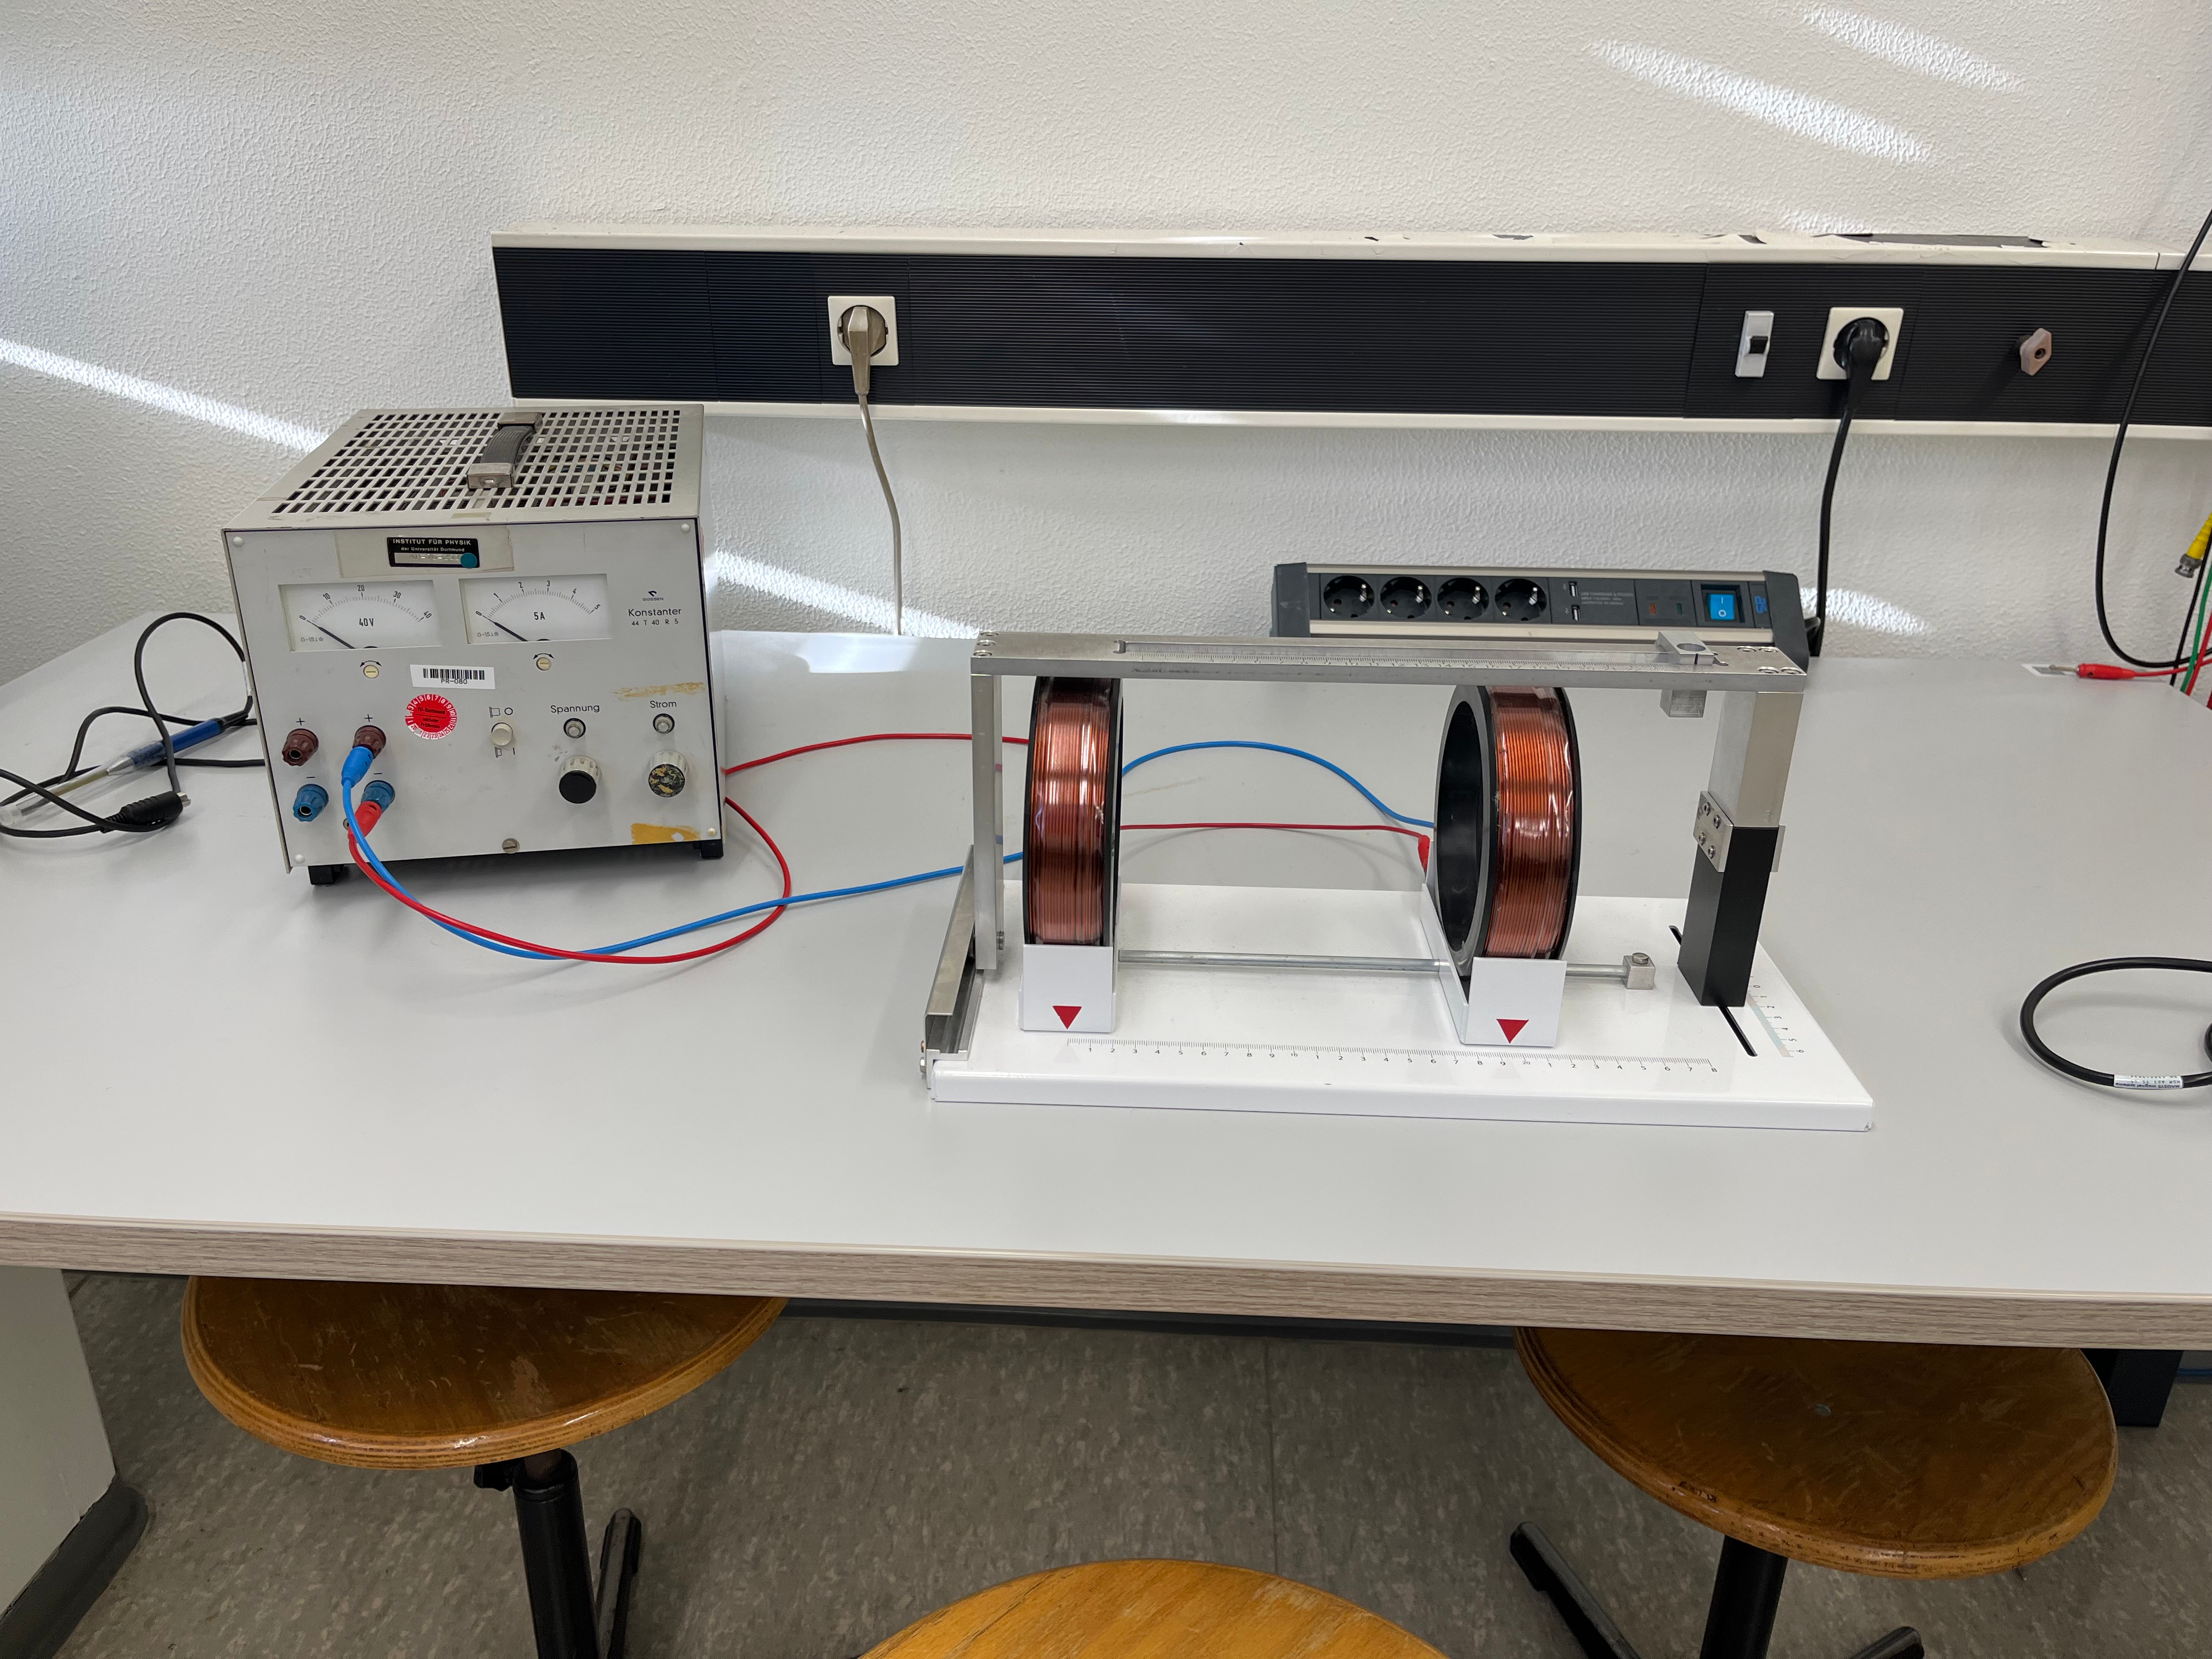
\includegraphics[width=.8\textwidth]{Pics/Img_Spulenpaar.png}
     \caption{Der Aufbau für die Helmholtzspulen, wobei eine verschiebbar ist. Zudem gibt es für die Hallsonde eine entprechende Vorrichtung.}

\end{figure}

\begin{figure}
    \centering
    \includegraphics[width=0.8\textwidth]{Pics/Aufbau2.jpg}
    \caption{Der Aufbau für den Toroid mit einem Luftspalt von 3 mm für die Hallsonde. }
\end{figure}
\section{Versuchsdurchführung}
In dem Versuch werden verschiedene Magnetfelder an multiplen Stellen in Spulenumgenung gemessen, von Einzelspulen, wie
auch von einem Spulenpaar und einer Ringspule.
\subsection{Magnetfeld von Spulen}
Zunächst wird eine lange Spule an ein Netzgerät angeschlossen und der Strom und die Spannung (unter Beachtung des
zulässigen Maximalstroms) hochgeregelt.
Das entstehende Magnetfeld wird in diesem Fall mit einer Longitudinalsonde gemessen, welche so aufgebaut wird, dass
das Feld auf der Spulenachse gemessen wird.
Im Anschluss wird das Gleiche mit einer kurzen Spule durchgeführt.
Es werden jeweils Werte innerhalb und außerhalb der Spule vermerkt und in einem x-B-Diagramm eingetragen.
\subsection{Magnetfeld eines Spulenpaares}
Nun wird das Netzgerät an das Spulenpaar angeschlossen, die Spulen sind in Reihe geschaltet.
Die Einstellungen für den Strom werden so gewählt, dass 5 A nicht überschritten werden.
Für drei verschiedene Abstände wird anschließend mit der transversalen Sonde das Magnetfeld ebenfalls inner- und
außerhalb des Spulenpaares gemessen und die Werte widerum in ein x-B-Diagramm übertragen.
\subsection{Hysteresekurve}
Zuletzt wird das Netzgerät an eine Ringspule angeschlossen und das Feld mit der Transversalsonde gemessen.
Dieses erfolgt in Abhängigkeit des herrschenden Spulenstroms.
Es werden sich verschiedene Messwerte für jeweilige Ströme notiert.




\end{document}